
\subsection{スマホアプリによる仮想ビーコンと実デバイスによるビーコンの併用}


% \begin{figure}[tbh]
%   \centering
%   \includegraphics[width=8cm]{image/hybrid.png}
%   \caption{仮想ビーコンと実デバイスによるビーコンの併用}
%   \label{multipleBPM}
% \end{figure}
% !!!!!!!!!!!!!!!!図2を利用する場合は言及する文章を書くこと 良い図を作る!!!!!!!!!!!!!!!!!!

実デバイスによるビーコンはメンバの利便性が低く可用性に問題がある.
可用性とは,メンバの在室情報が継続的に記録される能力と定義する.
実デバイスによるビーコンを利用する場合,高い可用性を維持するにはバッテリ交換に配慮する必要がある.
そこで既存研究ではバッテリ切れが発生した場合,管理者がメンバにSlackを用いて
通知しバッテリ交換を催促していた.
//これはメンバ全員のバッテリ交換を管理者が行うには困難であったためである.
しかし交換されない状況が存在した.
これは通知による催促が不確実かつ即時性がないためである.
通知は一定期間の在室がない場合にバッテリ切れの可能性があると見做して通知している.
そのため通知の正確性が低い上,バッテリ切れに対してタイムラグがある.
また交換作業がメンバに委ねられており,その手間による利便性が低くバッテリ切れの放置が発生した.


我々は実デバイスによるビーコンを導入する利点を維持した状態で欠点を解決させる方法としてスマホアプリによる仮想ビーコンと実デバイスによるビーコンの併用とそれに伴うAndroid向けのスマホアプリを作成した.
 現代においてスマートフォンは所持するインフラであり,本研究の対象とするユーザ層は可能な限りスマートフォンの電池状態に配慮する性質を持つ.
また,電池切れを外見上で判断不能なビーコンとは異なり画面表示などによって電池残量が判断可能である.

その性質を踏まえ実デバイスによるビーコンの利点であるユーザの意識的な記録動作を要しない点を維持するためにスマホアプリのバックグラウンド動作を行った.
 既存の研究では入退室を記録時に自身でスマホアプリを起動し記録する方式が採用されているが,我々の行っている実デバイスによるビーコンを携帯する方式の場合ユーザの記録動作なしで行われるためユーザの協力を得やすく,またヒューマンエラーを防止できる.
その利点を維持するために,スマホアプリを起動しビーコンの動作を開始した後は図2に示す通りスマートフォンの通知領域に動作状況を表示し,ユーザのそれ以上の操作を要しない.
通知領域への表示はビーコンとしての動作と連携しており, ビーコンの動作中は永続的に表示される.
よってスマホアプリが停止した場合もユーザによる判別が容易であるため,ユーザによる動作の再開が容易である.
これによって電池切れによる動作が停止する問題と実デバイスによるビーコンが専用のスマホアプリを要求する問題を解消している.

\begin{figure}[tbh]
  \centering
  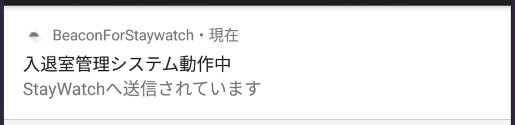
\includegraphics[width=8cm]{image/notify.jpg}
  \caption{通知領域による可視化}
  \label{multipleBPM}
\end{figure}



スマホアプリによる仮想ビーコンのみを利用する場合,様々な状況のユーザの継続した利用が困難であるため,実デバイスによるビーコンと併用できる仕様とした.
 普段から継続的に利用する滞在ウォッチユーザにとっては,実デバイスによるビーコンは先述の通り電池交換の手間がある.
スマホアプリはそのようなユーザにとっては,電池交換の手間がないため有用である.
 しかしスマホアプリのインストールに抵抗があるユーザやインストールができないユーザも想定される.
例としてはスマートフォンを所有していないユーザ,アプリの使用に伴う電池の消費が気になるユーザなどが上げられる.
 これらの問題は実デバイスによるビーコンとスマホアプリによる仮想ビーコンのハイブリッド化によって解決できる.
スマホアプリ内で利用するUUIDを実デバイスによるビーコンで使用するUUIDと同じ値に設定し同じユーザの在室情報を記録している.
この方法はスマートフォンか実デバイスによるビーコンのどちらかを所持していれば記録できるため継続的にデータを記録する観点から見ても有用である.

